At this point, we introduce a source to the wave equation. We consider a particle fixed on a circular orbit. A source on a circular orbit still emits radiation but requires an input of energy to the system to remain in a stationary orbit that does not inspiral. In this system, the self-force is counteracted by the force keeping the particle in its orbit. Imagine, in a science-fiction-like scenario, that the particle is a spacecraft with a compact object inside it, held in orbit by a thruster about a supermassive black hole. While this is not a physically reasonable scenario, it is a useful toy model for developing physical intuition about the effective source. 

\section{Self Force}




A test particle orbiting a black hole follows a geodesic, which is the path of extremal proper time. This is described by the geodesic equation,
\begin{equation}
\frac{d^2x^\mu}{d\tau^2}+\Gamma^\mu_{\rho\sigma}\frac{dx^\rho}{d\tau}\frac{dx^\sigma}{d\tau}=0
\end{equation}
where $\tau$ is the proper time and $\Gamma^\mu_{\rho\sigma}$ is the Christoffel symbol, given by~\cite{Carroll}
\begin{equation}
\Gamma^\sigma_{\mu\nu}=\frac{1}{2}g^{\sigma\rho}(\partial_\mu g_{\nu\rho}+\partial_\nu g_{\rho\mu} - \partial_\rho g_{\mu\nu})
\end{equation}

However, a black hole, of any size, is not a test particle. For an EMRI, if the full case of general relativity is considered and we do not simplify the problem to a scalar field, the additional force can be treated perturbatively in the mass ratio of the two particles. In the scalar case, the wave equation with a point particle source is simply written as a delta function source to the wave equation dependent upon the particle's position in time~\cite{WardellSelfForceReview}
\begin{eqnarray}
  \Box\Psi^{ret}=-4\pi q\int\delta_4(x,z(\tau^\prime))d\tau^\prime
\end{eqnarray}
In this equation, $\Box$ is the D'Alembertian and $z(\tau^\prime)$ is the evolving path of the source in space-time as a function of the particle's proper time. In the scalar approximation, the particle acts as a delta function point source, with a charge of $q$ and mass $m$. That charge may accelerate or evolve with time; see chapter~\ref{futurework}. 

The retarded field is singular at the location of the particle due to the delta function source. Singularities are computationally problematic. To regularize this singularity, a regular field is created through the use of an effective source.The regularized field, $\Psi^R$, is defined in terms of the retarded field with the Detweiler-Whiting singular field, $\tilde{\Psi}^S$, subtracted. 
\begin{equation}
\Psi^R=\Psi^{ret}-\tilde{\Psi}^S
\end{equation}


The wave equation on a curve spaced time is given an effective source that depends on the location of the particle in four space.

\begin{equation}
  \Box\Psi^R=S_{eff}
\end{equation}
Subtraction of the Detweiler-Whiting singular field cancels the source most precisely at the location of the singularity and approximately cancels it in its neighborhood. This leads to the definition of an effective source, $S_{eff}$, which is zero outside the neighborhood of the particle due to the world tube window function, $W$, shown in Figure~\ref{wtwindow}. Outside that region, the regularized field is equal to the retarded field.

\begin{equation}
S_{eff}=4\pi q\int\delta(x,z(\tau^\prime))d\tau^\prime-\Box(W\Psi^S)
\end{equation}

The Detweiler-Whiting singular field is derived from convolutions of retarded and advanced Greens functions appropriately symmetrized to select the singular part~\cite{detweiler_whiting}. It is perturbatively expanded in powers of the proper time along the particle's worldline~\cite{heffernan_ottewil_wardell_modesum_basisForCode} (Equation 3.7). The simulation currently incorporates the perturbative expansion to first order~\cite{heffernan_ottewil_wardell_modesum_basisForCode}, though a second order expansion to the Detweiler-Whiting singular field based upon a different approach is currently under devlopment~\cite{pound2ndOrderSelfForce2}. The self-force in a simulation can be computed is merely a gradient of the field itself~\cite{vega_wardell_diener_eff_source}. 



\section{World tube}
\begin{figure}
\includegraphics{worldTubeItself}
\caption{Spatial slice of the world tube window function.}
\label{wtwindow}
\end{figure}

The world tube window function around the particle carves out a spherical shell around the black hole, due to the use of spherical harmonics to compute the angular spatial dimensions in a 1+1 dimensional simulation. In my C++ code, the world tube extends throughout the entire tortoise region, ending at the transitions to the hyperboloidal regions. When calculating numerical fluxes at this boundary, it is necessary to account for both the coordinate transformations between either side of the boundary and the transformation between regular and retarded field.




\section{Comparison between C++ and Fortran codes}

I've performed a comparison between scalar particles on a circular orbit of radius 10M in Peter Diener's Fortran code~\cite{heffernan_ottewil_wardell_modesum_basisForCode}, implementing the same thing, and my C++ code. To roundoff precision, they agree, as evidenced by the near-machine-precision ($10^{-15}$) levels of agreement in both absolute and relative error that I achieve in Figures~\ref{circ1},~\ref{circ2},~\ref{circ3}, and~\ref{circ4}

\begin{figure}
  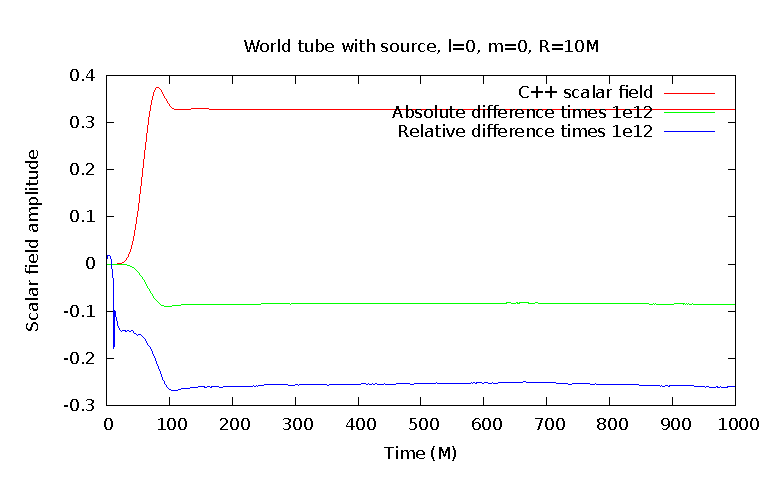
\includegraphics{wtcircl0m0}
  \caption{Comparison between Fortran and C++ scalar field along a line of sight for a particle on a circular orbit, l=0, m=0.}
  \label{circ1}
\end{figure}
\begin{figure}
  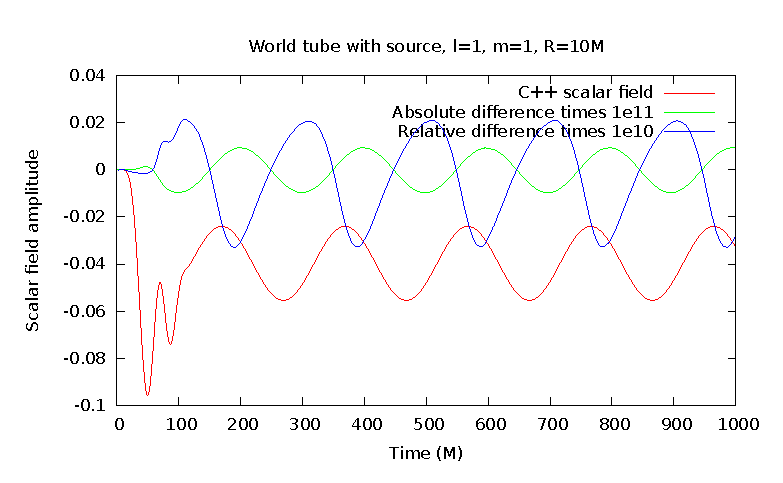
\includegraphics{wtcircl1m1}
  \caption{Comparison between Fortran and C++ l=1, m=1 scalar field along a line of sight for a particle on a circular orbit, l=1, m=1.}
  \label{circ2}
\end{figure}
\begin{figure}
  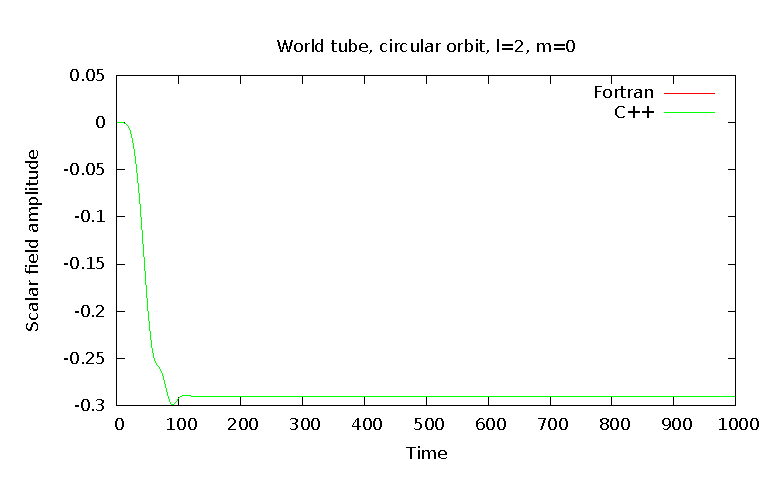
\includegraphics{wtcircl2m0}
  \caption{Comparison between Fortran and C++ l=2, m=0 scalar fields along a line of sight for a particle on a circular orbit, l=2, m=0.}
  \label{circ3}
\end{figure}
\begin{figure}
  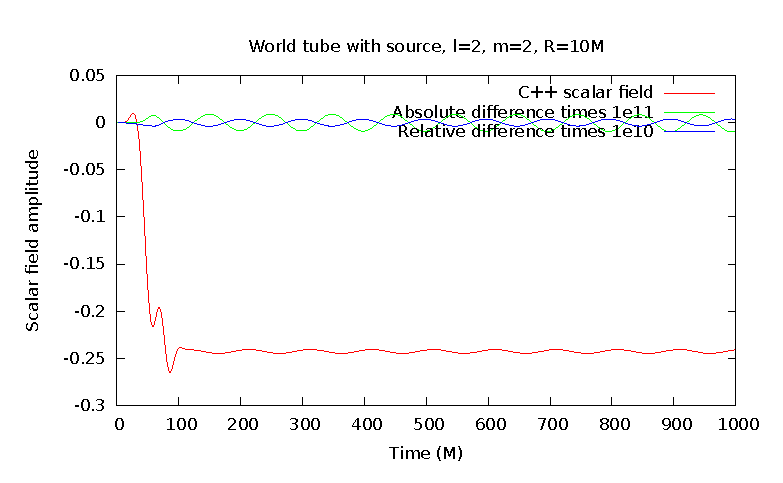
\includegraphics{wtcircl2m2}
  \caption{Comparison between Fortran and C++ l=2, m=2 scalar fields along a line of sight for a particle on a circular orbit, l=2, m=2.}
  \label{circ4}
\end{figure}
